\documentclass{standalone}
\usepackage{tikz}
\usetikzlibrary{patterns, positioning}


\begin{document}
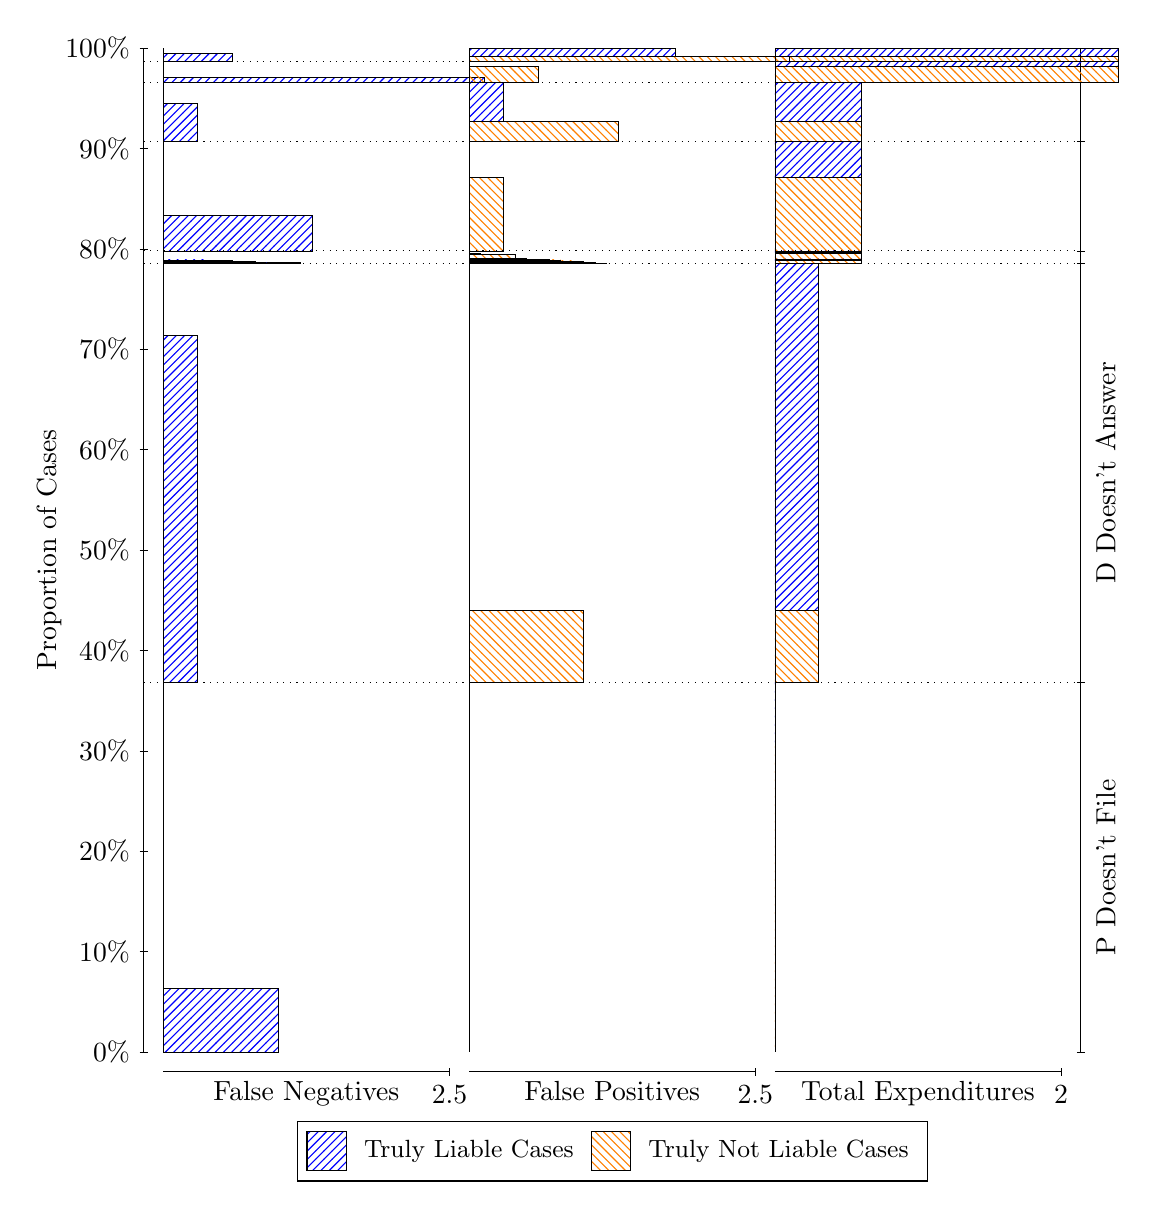
\begin{tikzpicture}
\draw[black, very thin] (1.5,1.75) -- (1.5,14.5);
\node[rotate=90, text=black, anchor=center] at (0.3, 8.125) {Proportion of Cases};
\draw[black, very thin] (1.45,1.75) -- (1.55,1.75);
\node[text=black, anchor=east] at (1.45, 1.75) {0\%};
\draw[black, very thin] (1.45,3.025) -- (1.55,3.025);
\node[text=black, anchor=east] at (1.45, 3.025) {10\%};
\draw[black, very thin] (1.45,4.3) -- (1.55,4.3);
\node[text=black, anchor=east] at (1.45, 4.3) {20\%};
\draw[black, very thin] (1.45,5.575) -- (1.55,5.575);
\node[text=black, anchor=east] at (1.45, 5.575) {30\%};
\draw[black, very thin] (1.45,6.85) -- (1.55,6.85);
\node[text=black, anchor=east] at (1.45, 6.85) {40\%};
\draw[black, very thin] (1.45,8.125) -- (1.55,8.125);
\node[text=black, anchor=east] at (1.45, 8.125) {50\%};
\draw[black, very thin] (1.45,9.4) -- (1.55,9.4);
\node[text=black, anchor=east] at (1.45, 9.4) {60\%};
\draw[black, very thin] (1.45,10.675) -- (1.55,10.675);
\node[text=black, anchor=east] at (1.45, 10.675) {70\%};
\draw[black, very thin] (1.45,11.95) -- (1.55,11.95);
\node[text=black, anchor=east] at (1.45, 11.95) {80\%};
\draw[black, very thin] (1.45,13.225) -- (1.55,13.225);
\node[text=black, anchor=east] at (1.45, 13.225) {90\%};
\draw[black, very thin] (1.45,14.5) -- (1.55,14.5);
\node[text=black, anchor=east] at (1.45, 14.5) {100\%};

\draw[black, very thin] (13.4,1.75) -- (13.4,14.5);
\draw[black, very thin] (13.35,1.75) -- (13.45,1.75);
\node[anchor=west] at (13.35, 1.75) {};
\draw[black, very thin] (13.35,6.4424) -- (13.45,6.4424);
\node[anchor=west] at (13.35, 6.4424) {};
\draw[black, very thin] (13.35,11.763) -- (13.45,11.763);
\node[anchor=west] at (13.35, 11.763) {};
\draw[black, very thin] (13.35,11.925) -- (13.45,11.925);
\node[anchor=west] at (13.35, 11.925) {};
\draw[black, very thin] (13.35,13.31) -- (13.45,13.31);
\node[anchor=west] at (13.35, 13.31) {};
\draw[black, very thin] (13.35,14.063) -- (13.45,14.063);
\node[anchor=west] at (13.35, 14.063) {};
\draw[black, very thin] (13.35,14.329) -- (13.45,14.329);
\node[anchor=west] at (13.35, 14.329) {};
\draw[black, very thin] (13.35,14.5) -- (13.45,14.5);
\node[anchor=west] at (13.35, 14.5) {};

\draw[black, very thin, pattern color=blue, pattern=north east lines] (1.75,1.75) rectangle (3.2033,2.5577);
\draw[black, very thin, pattern color=orange, pattern=north west lines] (1.75,2.5577) rectangle (1.75,6.4424);
\draw[black, very thin, pattern color=blue, pattern=north east lines] (1.75,6.4424) rectangle (2.186,10.853);
\draw[black, very thin, pattern color=orange, pattern=north west lines] (1.75,10.853) rectangle (1.75,11.763);
\draw[black, very thin, pattern color=blue, pattern=north east lines] (1.75,11.763) rectangle (3.494,11.775);
\draw[black, very thin, pattern color=blue, pattern=north east lines] (1.75,11.775) rectangle (3.3487,11.777);
\draw[black, very thin, pattern color=blue, pattern=north east lines] (1.75,11.777) rectangle (3.2033,11.78);
\draw[black, very thin, pattern color=blue, pattern=north east lines] (1.75,11.78) rectangle (3.058,11.78);
\draw[black, very thin, pattern color=blue, pattern=north east lines] (1.75,11.78) rectangle (3.058,11.78);
\draw[black, very thin, pattern color=blue, pattern=north east lines] (1.75,11.78) rectangle (2.9127,11.789);
\draw[black, very thin, pattern color=blue, pattern=north east lines] (1.75,11.789) rectangle (2.7673,11.792);
\draw[black, very thin, pattern color=blue, pattern=north east lines] (1.75,11.792) rectangle (2.622,11.801);
\draw[black, very thin, pattern color=blue, pattern=north east lines] (1.75,11.801) rectangle (2.4767,11.806);
\draw[black, very thin, pattern color=blue, pattern=north east lines] (1.75,11.806) rectangle (2.3313,11.808);
\draw[black, very thin, pattern color=orange, pattern=north west lines] (1.75,11.808) rectangle (1.75,11.925);
\draw[black, very thin, pattern color=blue, pattern=north east lines] (1.75,11.925) rectangle (3.6393,12.376);
\draw[black, very thin, pattern color=orange, pattern=north west lines] (1.75,12.376) rectangle (1.75,13.31);
\draw[black, very thin, pattern color=blue, pattern=north east lines] (1.75,13.31) rectangle (2.186,13.799);
\draw[black, very thin, pattern color=orange, pattern=north west lines] (1.75,13.799) rectangle (1.75,14.063);
\draw[black, very thin, pattern color=blue, pattern=north east lines] (1.75,14.063) rectangle (5.8193,14.127);
\draw[black, very thin, pattern color=orange, pattern=north west lines] (1.75,14.127) rectangle (1.75,14.329);
\draw[black, very thin, pattern color=blue, pattern=north east lines] (1.75,14.329) rectangle (2.622,14.436);
\draw[black, very thin, pattern color=orange, pattern=north west lines] (1.75,14.436) rectangle (1.75,14.5);
\draw[black, very thin, pattern color=orange, pattern=north west lines] (5.6333,1.75) rectangle (5.6333,5.6347);
\draw[black, very thin, pattern color=blue, pattern=north east lines] (5.6333,5.6347) rectangle (5.6333,6.4424);
\draw[black, very thin, pattern color=orange, pattern=north west lines] (5.6333,6.4424) rectangle (7.0867,7.3532);
\draw[black, very thin, pattern color=blue, pattern=north east lines] (5.6333,7.3532) rectangle (5.6333,11.763);
\draw[black, very thin, pattern color=orange, pattern=north west lines] (5.6333,11.763) rectangle (7.3773,11.765);
\draw[black, very thin, pattern color=orange, pattern=north west lines] (5.6333,11.765) rectangle (7.232,11.774);
\draw[black, very thin, pattern color=orange, pattern=north west lines] (5.6333,11.774) rectangle (7.0867,11.789);
\draw[black, very thin, pattern color=orange, pattern=north west lines] (5.6333,11.789) rectangle (6.9413,11.796);
\draw[black, very thin, pattern color=orange, pattern=north west lines] (5.6333,11.796) rectangle (6.796,11.809);
\draw[black, very thin, pattern color=orange, pattern=north west lines] (5.6333,11.809) rectangle (6.6507,11.811);
\draw[black, very thin, pattern color=orange, pattern=north west lines] (5.6333,11.811) rectangle (6.5053,11.818);
\draw[black, very thin, pattern color=orange, pattern=north west lines] (5.6333,11.818) rectangle (6.36,11.824);
\draw[black, very thin, pattern color=orange, pattern=north west lines] (5.6333,11.824) rectangle (6.2147,11.88);
\draw[black, very thin, pattern color=blue, pattern=north east lines] (5.6333,11.88) rectangle (5.924,11.883);
\draw[black, very thin, pattern color=blue, pattern=north east lines] (5.6333,11.883) rectangle (5.7787,11.888);
\draw[black, very thin, pattern color=blue, pattern=north east lines] (5.6333,11.888) rectangle (5.6333,11.925);
\draw[black, very thin, pattern color=orange, pattern=north west lines] (5.6333,11.925) rectangle (6.0693,12.858);
\draw[black, very thin, pattern color=blue, pattern=north east lines] (5.6333,12.858) rectangle (5.6333,13.31);
\draw[black, very thin, pattern color=orange, pattern=north west lines] (5.6333,13.31) rectangle (7.5227,13.573);
\draw[black, very thin, pattern color=blue, pattern=north east lines] (5.6333,13.573) rectangle (6.0693,14.063);
\draw[black, very thin, pattern color=orange, pattern=north west lines] (5.6333,14.063) rectangle (6.5053,14.265);
\draw[black, very thin, pattern color=blue, pattern=north east lines] (5.6333,14.265) rectangle (5.6333,14.329);
\draw[black, very thin, pattern color=orange, pattern=north west lines] (5.6333,14.329) rectangle (9.7027,14.393);
\draw[black, very thin, pattern color=blue, pattern=north east lines] (5.6333,14.393) rectangle (8.2493,14.5);
\draw[black, very thin, pattern color=orange, pattern=north west lines] (9.5167,1.75) rectangle (9.5167,5.6347);
\draw[black, very thin, pattern color=blue, pattern=north east lines] (9.5167,5.6347) rectangle (9.5167,6.4424);
\draw[black, very thin, pattern color=orange, pattern=north west lines] (9.5167,6.4424) rectangle (10.062,7.3532);
\draw[black, very thin, pattern color=blue, pattern=north east lines] (9.5167,7.3532) rectangle (10.062,11.763);
\draw[black, very thin, pattern color=orange, pattern=north west lines] (9.5167,11.763) rectangle (10.607,11.799);
\draw[black, very thin, pattern color=blue, pattern=north east lines] (9.5167,11.799) rectangle (10.607,11.821);
\draw[black, very thin, pattern color=orange, pattern=north west lines] (9.5167,11.821) rectangle (10.607,11.892);
\draw[black, very thin, pattern color=blue, pattern=north east lines] (9.5167,11.892) rectangle (10.607,11.908);
\draw[black, very thin, pattern color=orange, pattern=north west lines] (9.5167,11.908) rectangle (10.607,11.919);
\draw[black, very thin, pattern color=blue, pattern=north east lines] (9.5167,11.919) rectangle (10.607,11.925);
\draw[black, very thin, pattern color=orange, pattern=north west lines] (9.5167,11.925) rectangle (10.607,12.858);
\draw[black, very thin, pattern color=blue, pattern=north east lines] (9.5167,12.858) rectangle (10.607,13.31);
\draw[black, very thin, pattern color=orange, pattern=north west lines] (9.5167,13.31) rectangle (10.607,13.573);
\draw[black, very thin, pattern color=blue, pattern=north east lines] (9.5167,13.573) rectangle (10.607,14.063);
\draw[black, very thin, pattern color=orange, pattern=north west lines] (9.5167,14.063) rectangle (13.877,14.265);
\draw[black, very thin, pattern color=blue, pattern=north east lines] (9.5167,14.265) rectangle (13.877,14.329);
\draw[black, very thin, pattern color=orange, pattern=north west lines] (9.5167,14.329) rectangle (13.877,14.393);
\draw[black, very thin, pattern color=blue, pattern=north east lines] (9.5167,14.393) rectangle (13.877,14.5);
\draw[black, dotted] (1.5,6.4424) -- (13.4,6.4424);
\draw[black, dotted] (1.5,11.763) -- (13.4,11.763);
\draw[black, dotted] (1.5,11.925) -- (13.4,11.925);
\draw[black, dotted] (1.5,13.31) -- (13.4,13.31);
\draw[black, dotted] (1.5,14.063) -- (13.4,14.063);
\draw[black, dotted] (1.5,14.329) -- (13.4,14.329);
\draw[black, very thin] (1.75,1.5) -- (5.3833,1.5);
\node[text=black, anchor=north] at (3.5667, 1.5) {False Negatives};
\draw[black, very thin] (5.3833,1.45) -- (5.3833,1.55);
\node[text=black, anchor=north] at (5.3833, 1.45) {2.5};

\draw[black, very thin] (5.6333,1.5) -- (9.2667,1.5);
\node[text=black, anchor=north] at (7.45, 1.5) {False Positives};
\draw[black, very thin] (9.2667,1.45) -- (9.2667,1.55);
\node[text=black, anchor=north] at (9.2667, 1.45) {2.5};

\draw[black, very thin] (9.5167,1.5) -- (13.15,1.5);
\node[text=black, anchor=north] at (11.333, 1.5) {Total Expenditures};
\draw[black, very thin] (13.15,1.45) -- (13.15,1.55);
\node[text=black, anchor=north] at (13.15, 1.45) {2};

\node[text=black, centered, rotate=90] at (13.72, 4.0962) {P Doesn't File};
\node[text=black, centered, rotate=90] at (13.72, 9.1028) {D Doesn't Answer};






\draw (7.449999999999999,1.5) node[draw=none] (baseCoordinate) {};
\begin{scope}[align=center]
        \matrix[scale=0.5, draw=black, below=0.5cm of baseCoordinate, nodes={draw}, column sep=0.1cm]{
            \node[rectangle, draw, minimum width=0.5cm, minimum height=0.5cm, pattern color=blue, pattern=north east lines] {}; &
            \node[draw=none, font=\small, text=black] (B) {Truly Liable Cases}; &
            \node[rectangle, draw, minimum width=0.5cm, minimum height=0.5cm, pattern color=orange, pattern=north west lines] {}; &
            \node[draw=none, font=\small, text=black] (B) {Truly Not Liable Cases}; \\
            };
\end{scope}

\end{tikzpicture}
\end{document}